\documentclass[a4paper,12pt]{report}
\usepackage{graphicx}
\usepackage{subcaption}
\usepackage{amsmath}
%\usepackage{amsthm}
\usepackage[bottom]{footmisc}
\usepackage{apacite}
\usepackage{pdfpages}
\usepackage{ntheorem}
\theoremseparator{:}
\newtheorem{hyp}{Hypothesis}
\newtheorem{prop}{Proposition}

%\theoremstyle{definition}
\newtheorem{ass}{Assumption}[section]

%\usepackage[nottoc]{tocbibind}
%\usepackage{biblatex}
\usepackage{chngcntr}
\counterwithout{equation}{chapter} 
\counterwithout{figure}{chapter} % remove chapter number
\counterwithout{table}{chapter}

\usepackage[T1]{fontenc}
\usepackage{titlesec, blindtext, color}
\definecolor{gray75}{gray}{0.75}
\newcommand{\hsp}{\hspace{20pt}}
\titleformat{\chapter}[hang]{\Huge\bfseries}{\thechapter\hsp\textcolor{gray75}{|}\hsp}{0pt}{\Huge\bfseries}

\begin{document}

\setlength{\parindent}{0pt}
\setlength{\parskip}{6pt}















\chapter{Results}
\section{Output}
\subsection{Typical simluations}

%%%%%%%%%%%% CHANGE PLAN ?
%%% intro : this section = 
    %%% and do math ===> NE not ESS...
%% exog ... either in two or one...
%% ss2

A simulation = .... show picture : genes, field, network
=> show two picture, one with also model SS2
Genes = weighted over 8 bits : values between $0$ and $2^8 - 1$

this should be much longer


so as figures don't run into one another... 

otherwise learn to skip pages...

Mostly will be working with average for relative value for genes over the pop / after a lot of time
One experiment => results for four genes
Typically (unless specified overwise), values averaged over 30 experiments


MATH = NE.... => en fait on en a deja parle en section 2.... 
    => MODIF SECTION II plutot...

\subsection{Remembered Heroes}
\label{ss:RH}
These output values are precise to the percentage point. 
For $\bf{SelfSacrifice}$ this poses a problem, as final values are expected to be relatively
small - with typical parameter values (as in \textbf{section 2}), average probability of self-sacrifice
 is capped at 2-3\%.

For this reason, simulations also kept track of $\bf{RememberedHeroes}$, a measure for the number of heroes 
in the live memory of a society. At each simulation step (year), the number of "voluntary" martyrs was computed
 by subtracting the expected number of martyrs which could be solely attributable to mutations in a population
 that did not engage in self-sacrifice. These were added to the number of heroes which could be assumed to have
 been \emph{witnessed} by (alive) individuals in the population. In a given year, $\bf{RememberedHeroes}$ corresponds
 to the number of heroes witnessed by at least \emph{RemThreshold} percent of the population (5 \% in practice).
 In situations where self-sacrificial behavior can be said to be absent, $\bf{RememberedHeroes}$ is close to 0
 (e.g. when \emph{Admiration} is null in the first model under).

\section{Exogenous model: simulation outputs}


%%%%%%%% CHANGE : model interpretation for f...
%%% truc cool: si on trouvait a la fin f = Rmax / p...


\subsection{Main results}

\begin{figure}[h]
\centering
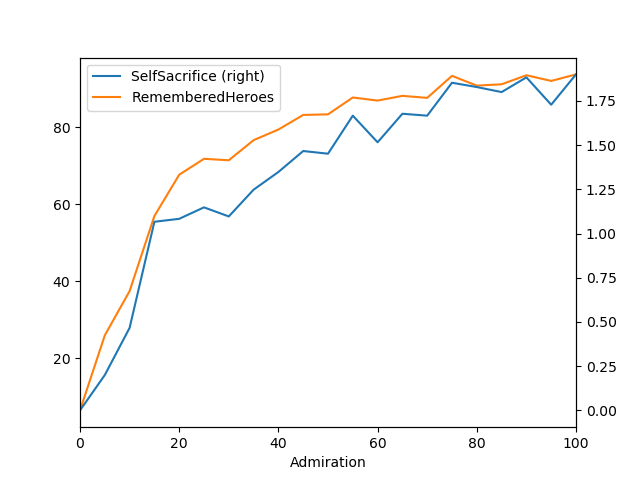
\includegraphics[width=1\textwidth]{RGT_10}
\caption{$\bf{SelfSacrifice}$ and $\bf{RememberedHeroes}$, as a function of \emph{Admiration} (typical parameter values).}
\label{fig:RGT_10}
\end{figure}



\textbf{Figure \ref{fig:RGT_10}} shows results obtained by averaging over 30 simulations, according to the \emph{Admiration}
 parameter (all others being kept constant at the previously described values). As could be expected, $\bf{RememberedHeroes}$
 rises from 0 with \emph{Admiration}, quickly reaching two thirds of its maximum value of under 100 heroes when
 \emph{Admiration} exceeds 20. 
 
 $\bf{SelfSacrifice}$ follows similar dynamics, with values ranging between 0 and 2\% (values to a higher precision than
 the percentage point being obtained artificially by averaging over experimental results). These values are far from negligible:
 for a typical population of 200, we expect an average of (almost) 4 martyrs each year.
 Such collective behavior is captured here by individuals all bearing similar genetic probability $P$
 of self-sacrifice at equilibrium (and obtaining similar $\bf{Reproductive\_points}$ in the 
 long-term), as seen on \textbf{Figure \ref{fig:Snap}}. 
 
 \begin{figure}[h]
    \centering
    \begin{subfigure}[b]{0.3\linewidth} 
        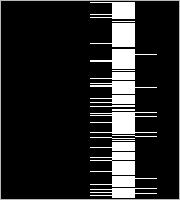
\includegraphics[width=\linewidth, height =\linewidth]{Exo_Genome}
        \caption{Genetic values}
    \end{subfigure}
    \begin{subfigure}[b]{0.3\linewidth}
        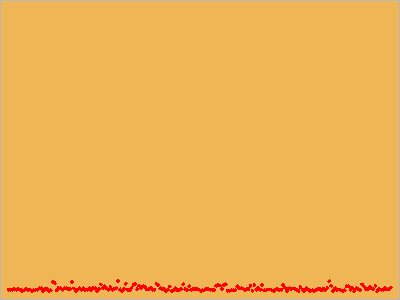
\includegraphics[width=\linewidth, height = \linewidth]{Exo_Field}
        \caption{Reproductive points}
    \end{subfigure}
    \caption{Snapshot of individual values, \emph{A=50}. An individual's genome is represented by a horizontal line on the left: here most bear a $\bf{SelfSacrifice}$ gene
    of relative value $\frac{2^2}{2^8-1}$ (around $1.6\%$). Individuals (horizontal axis) and their reproductive points (vertical) are represented on the right.}
    \label{fig:Snap}
    \end{figure}


 However, one can also imagine the collectively equivalent situation where only a small fraction $f$ of individuals
 engage in self-sacrificial behavior with higher probability $p$ (with $P = f*p$), to the much more
 significant benefit of their families (see \textbf{Section \ref{sec_exo_math}}).

\subsection{Influence of \emph{ReproGainsThreshold} $RGT$}

\begin{figure}[h]
    \centering
    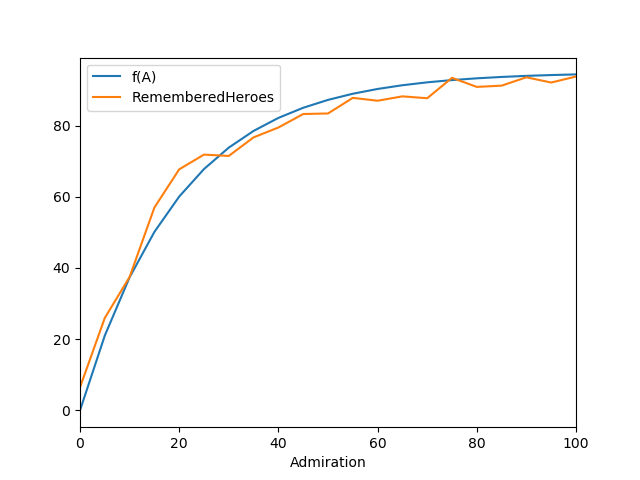
\includegraphics[width=0.6\textwidth]{f_rgt10}
    \caption{$\bf{RememberedHeroes}$ and corresponding optimal $f$ as functions of 
    \emph{Admiration}, for $RGT=10$ ($C=95, \tau = 20$).}
    \label{fig:f_10}
    \end{figure}

As a function of \emph{Admiration}, $\bf{RememberedHeroes}$ resembles a function of the form:
$f_{C,\tau}(t) = C*(1-exp(-t/\tau))$.
% Com sur la forme de la fonction ? Par ex: selection d'une allele, cf Nettle p80
% ou radioactive decay / pop growth with ...
Very approximately\footnote{By choosing optimal C and $\tau$ at a precision of 5 units;
the idea here being simply to get a "feel" for overall variation with $A$. Optimal parameters are the
ones for which Euclidean distance is minimal.},
it can best be approached by a function of this form with parameters $C=95$ and $\tau = 20$, as visible
on \textbf{Figure \ref{fig:f_10}}.

\begin{figure}[h]
    \centering
    \begin{subfigure}[b]{0.4\linewidth} 
        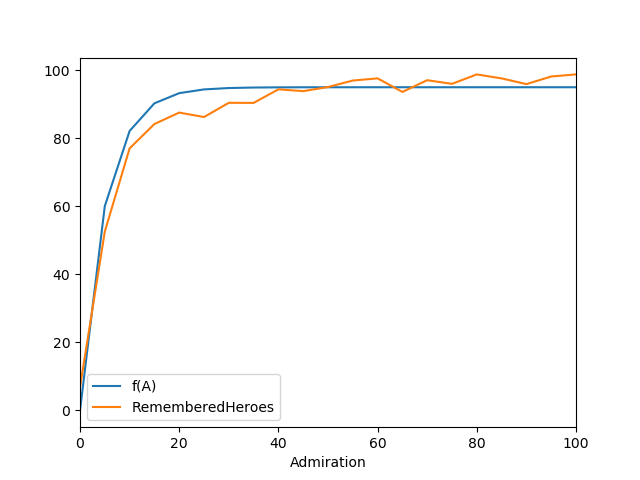
\includegraphics[width=\linewidth]{f_rgt5}
        \caption{$RGT=5$ ($C=95,\tau=5$)}
    \end{subfigure}
    \begin{subfigure}[b]{0.4\linewidth}
        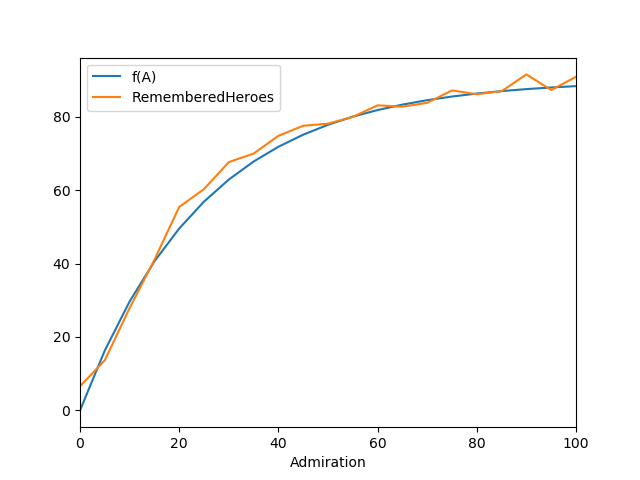
\includegraphics[width=\linewidth]{f_rgt20}
        \caption{$RGT=20$ ($C=90,\tau=25$)}
    \end{subfigure}
    \caption{$\bf{RememberedHeroes}$ and $f$ for $RGT=5, 20$}
    \label{fig:RGT5-20}
    \end{figure}

The key parameter governing relative growth of $\bf{RememberedHeroes}$\footnote{
This output's absolute value is arbitrary, chosen according to \emph{RemThreshold} in
order to provide for visible variations (see \textbf{Section \ref{ss:RH}}).
} thus appears to be one equal to two times
\emph{ReproGainsThreshold}. The importance of $RGT$ is not surprising since it plays
the crucial role of defining the unit in which $\bf{Reproductive\_points}$ are counted.  
The relationship between $RGT$ and final results is however non-trivial, since 
variation according to $A$ for $RGT=5$ (resp. $RGT=20$) are best captured by $\tau=5$
(resp. $\tau=25$), as visible on \textbf{Figure \ref{fig:RGT5-20}}; suggesting perhaps
a quadratic relationship between $RGT$ and $\tau$. \textbf{Section \ref{ss: exo_existence}}
returns to this issue.
%%% A MODIF : provides a charac for minimal ESS > 0... et plus si affinites?

\subsection{Variation with \emph{SacrificeHeredity} $h$}

%%% Au moins le graphe A = 50 vs h... => et donc ?
Contrary to what could be expected, h -> 1 is a problem: probs because pop = too small
and all end up with same h... - as shown by simu // because same family ? (or just expected in LT?)
h = 0 discontinuity = expected

\begin{figure}[h]
    \centering
    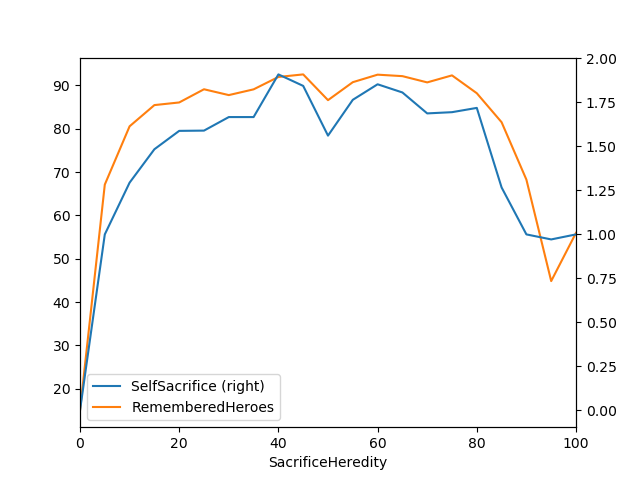
\includegraphics[width=0.6\textwidth]{Hered_a50}
    \caption{}
    \label{fig:h}
    \end{figure}

%%%%%%%%%%%%%% h =50 < ? ===> va avec l'hyp de la concurrence... meme shares...

%%% j'ai aussi teste pour A variant... mais osef (h 0 /25 /75 / 100)

%%% A VENIR : test sur pop = tres gros...
%%%%%%%%% test un peu sur gros = 1000 : ca decroit aussi, meme si je sais pas si c'est autant
%% (test entre 80 et 100...)
%%%%% cf Grospop_h.png

\subsection{Variation with \emph{ReproductionRate} $r$}
%%% Duh, with N... // and also relationship p and r visibly => cf section 1.3.3.

\begin{figure}[h]
    \centering
    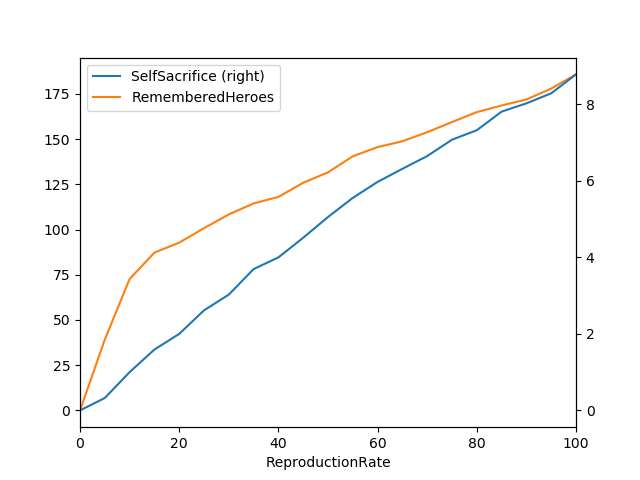
\includegraphics[width=0.6\textwidth]{Repro}
    \caption{}
    \label{fig:r}
    \end{figure}
%%% DUH : 0 if r = 0, since population disappears after one generation...
%(step 90 here... bizarre j'ai mis age max = 100 ?) --> oui, ou pas d'influence
%oui...

    \begin{figure}[h]
        \centering
        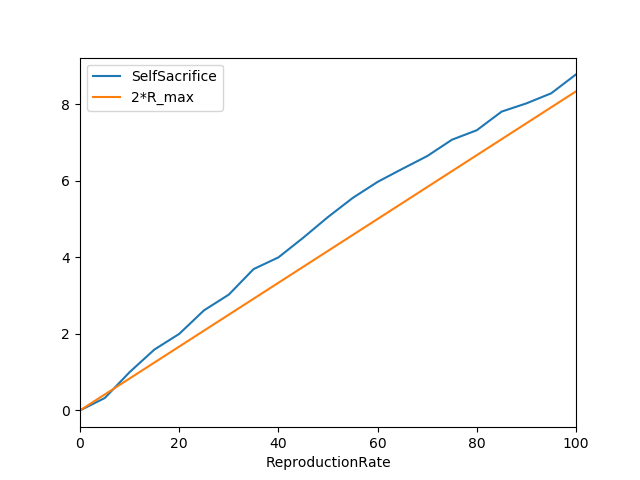
\includegraphics[width=0.6\textwidth]{Repro_magie}
        \caption{}
        \label{fig:r_magie}
        \end{figure}
%%% OOPS: pas tant de la magie: c'est R_max / 50 !
%%%%%%%%%%%%%%%%%%%%%%%%% donc quoi, A ?
            %%% non (
%%% ne depend pas de RGT non plus
%%% ni d'age max

%%%% il reste S, N, GeneLength, HEREDITY ??

%%%%%%%%%% plus tester avec r / 1+r * (1 - S log (1_S)/ 1+S))...
%%%%%%%%%%%%%%%%%%%%%%%%%%%%%%%%%% !!


%%%%% Remarque : RH et SS ne dependent pas de l'Age... (cf Exogene/)
%%% donc l'erreur de para ne devrait pas changer grand chose
%%% par contre mon resultat final = ?????


\section{Exogenous model: mathematical proof of concept}
\label{sec_exo_math}
%%% BONUS : here add f << 1 : using equation on A * ... / f < RGT...


%%%%%%%%%%%% RAJOUTER TOUS LES EXPECTEDE VALUE C'est plus simple... 
%%% ca evitera de se repeter...

\subsection{Simplifying assumptions}
%%% subsubsection?
\label{ss:exm_eq}
Individuals live to a maximum of \emph{AgeMax} $M$ years, fixed at 40 here. 
 Expected lifespan is lower however, as individuals face random accidents
 (in a wide sense) and is equal to $\alpha*M$, where $\alpha$ captures
 the effects of natural selection. In this model, all individuals face the same $\alpha$, but
 may obtain differing reproductive opportunities ($\bf{Selectivity}$ mode).

Individuals who engage in self-sacrificial behavior with probability $p$
 shorten their expected lifespan by a multiplicative factor of (see \textbf{Appedix \ref{beta}}):
 
\begin{equation}
 \beta(p) = \frac{(1-p) - (1-p)^{(M+1)}}{p*M} 
\label{eq_beta}
\end{equation}

As such, their reproductive window is shorter on average, which should lead to the disappearance of
self-sacrificial behavior - unless this is compensated by increased reproductive opportunities. 
 
In order to attempt to attain a mathematical proof of concept, a number of \emph{simplifying assumptions}
were made, which stand in contrast to how the previous simulation is actually played:

\begin{ass}[A\ref{ass:p_fixed}] \label{ass:p_fixed}
    Probability of self-sacrifice $p$ is fixed; 
    what varies is the proportion of agents who engage
    in such a strategy $f$.
    \end{ass}

\begin{ass}[A\ref{ass:domi}] \label{ass:domi}
    Self-sacrifice is related to a dominant schematic "allele": the children
    of a would-be martyr and another individual are would-be
    martyrs for yearly probability $p$
    (and not $\frac{p}{2}$).
    \end{ass}

\begin{ass}[A\ref{ass:p_large}] \label{ass:p_large}
    $p$ and $M$ are large enough for such agents to be all but assured that they will die laying down
    their lives for the sake of the group (and not in another way) which can be written as:
    $(1-p)^M \ll 1$ and $p \gg \alpha$.
    \end{ass}

\begin{ass}[A\ref{ass:gene}] \label{ass:gene}
    Generations do not overlap; individuals are granted their lifetime reproductive potential $R$
    at birth.
    \end{ass}
    
Even though these assumptions set our mathematical model apart from the simulation, we still
expect some connection between final results in both cases. In particular, population probability of 
self-sacrifice $p^{sim}$ in the first case should resemble the one here which is equal to
$p*f$. Since mutation rate (0.5\%) and previous results were small (1-2\%) (and $p$ is assumed not to be here),
let us also assume:

\begin{ass}[A\ref{ass:mut}] \label{ass:mut}
    Mutation rate is negligible.
    \end{ass}

\begin{ass}[A\ref{ass:f_small}] \label{ass:f_small}
    Proportion of would-be martyrs remains negligible: $f \ll 1$.
    \end{ass}


\subsection{Mathematical characterization of equilibrium}

Let us start from a situation where there are no martyrs in recent memory, and a
proportion $f_0$ of individuals born with a propensity to martyrdom, captured by $p$.
These individuals obtain on average 
$\alpha*\beta(p)*M*r$ offspring each,
when others obtain $\alpha*M*r$, where $r$ is the population-level \emph{ReproductionRate}. 

Following (A\ref{ass:p_large}), a would-be martyr's child $i$ obtains
reproductive potential $R^i>r$.
Martyrs children are in proportion $f_1$ in their generation (A\ref{ass:gene}).
Since $f_{1} \ll 1$ (A\ref{ass:f_small}), $R^i$ can be assumed to be the same
for all such children, and will be written
$R_+(A,f_1)$, where $A$ is \emph{Admiration} (we neglect the possibility of 
individuals being born from two would-be martyrs).
Children of non-would be martyrs obtain on average
$R_-$ which, for the same reason, can be approximated to $r$ (A\ref{ass:f_small}).

Since self-sacrifice is assumed to be heritable, 
these second-generation martyrs obtain on average $\alpha*\beta(p)*M*R_+(A,f_1)$
children, who obtain $\alpha*\beta(p)*M*R_+(A,f_2)$ children, etc. Non-martyrs
continue to obtain $\alpha*M*r* children$.
Thus, (potential) equilibrium between $f\ll 1$ would-be martyrs and $1-f$ others is
characterized by:
\begin{equation}
    R_+(A,f)*\beta(p) = r
\label{eq:grandchildren}
\end{equation}
%% le environ egal devient egal...


\subsection{Necessary condition for an ESS}
\label{ss: exo_existence}

Let $N$ be equal to \emph{PopulationSize}, implicitly assumed to be large here (since $f$
is negligible).

In the spirit of (A\ref{ass:gene}), let us assume
that total social admiration is borne by the children of non-heroes, and is thus equal to
$A*(1-f)*N$ at potential equilibrium. 
For children of martyrs, two situations are possible:

\begin{itemize}
\item either $\frac{A*(1-f)*N}{fN} < RGT$, and 
all receive reproductive potential $r$;
\item or $\frac{A*(1-f)*N}{fN} \geq RGT$, and all receive $R_{+}(A,f)>r$.
\end{itemize}

Thus, self-sacrifice as characterized by $p>0$ and $f>0$ can only constitute an ESS if:
\begin{equation}
    \label{eq:min_ESS_e}
    A \geq A_{min}=\frac{RGT*f}{1-f}
\end{equation}

A condition which, since we assumed $f \ll 1$, is highly likely to be met.
%ca existe tjs un ESS ? Pas sur, c'est plutot l'eq de Nash en strat mixte...

\subsection{Equilibrium value}

%%% COMMENCER ICI / dans l'annexe correspondante : calcul de p a l'eq... (sachant f petit...)
%% => pb pour l'AN ???
As shown in \textbf{Appendix \ref{ss:R+}}, a first-order approximation of $R_+$
in the latter case is ($S$ is equal to \emph{Selectivity}):
\begin{equation}
    R_+(A,f) = \frac{S*r}{log(1+S)} * (1 - \frac{S*f)}{2})
\label{eq:R+}
\end{equation}
Using (\ref{eq:grandchildren}), we deduce that both envisioned strategies are equivalent if
and only if:
\[\frac{Sr}{log(1+S)}(1-\frac{S*f}{2})\beta(p)=r  \]
\begin{equation}
    \label{eq:trinome_beta}
    \iff f = \frac{2}{S}*(1-\frac{log(1+S)}{\beta(p)*S})
\end{equation}
%%%%%%%%%%%%%%%%%%%%%%%%%%%%%%%%%%% WTF ON TROUVE f<0...

%%%%% a refaire : RECOMMENCE ICI
%%%% SINON TRICHE = repartir avec les beta comme avant,
%%% ou p n'est pas heritable... --- serait mieux pour les calculs...


Since $(1-p)^M \ll 1$ (A\ref{ass:p_large}),
\[\beta(p) \approx \frac{1-p}{p*M}\]

Which yields:
\begin{equation}
f \approx f_{eq}(p) = \frac{2}{S}*(1-\frac{p*log(1+S)}{(1-p)*S)})
\end{equation}

\begin{figure}[h]
    \centering
    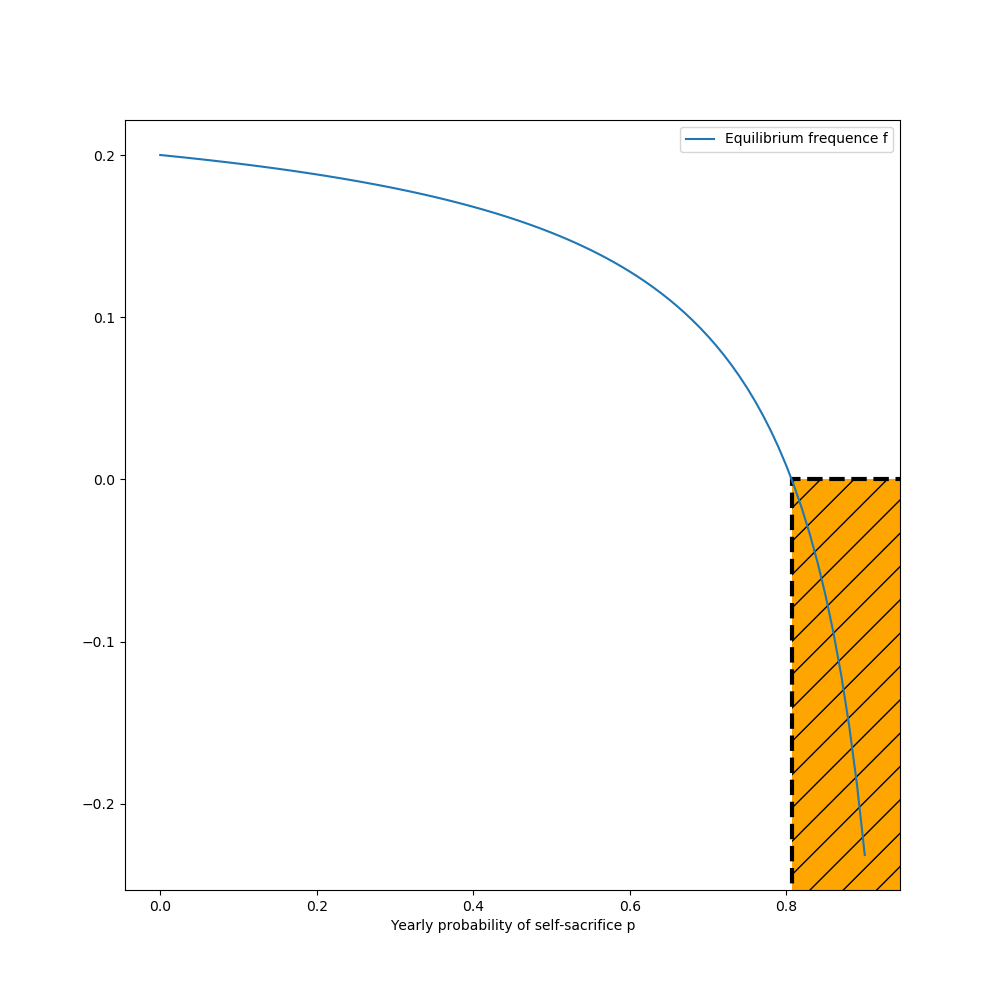
\includegraphics[width=0.6\textwidth]{Exo_f_ESS}
    \caption{$f_{eq}(p)$. Forbidden values ($p \geq p_{max}$) are 
    represented by the orange rectangle.}
    \label{fig:f_ESS}
    \end{figure}

As shown by \textbf{Figure \ref{fig:f_ESS}}, $f_{eq}(p)$ is positive for
$p < p_{max} = \frac{S}{log(1+S)+S} \approx 0.81\%$ for S = 10. 

\begin{prop}
    %%%% Moche le itemize ?
Under assumptions (A\ref{ass:p_fixed}-\ref{ass:f_small}), for:
\begin{itemize}
    \item $A \geq A_{min}$ ;
    \item and $p \leq p_{max}$ ;
\end{itemize}
a self-sacrifice Nash equilibrium (NE) exists, where a first-order
approximation of proportion of would-be martyrs at equilibrium is:
\[f(S,p) = \frac{2}{S}*(1-\frac{p*log(1+S)}{(1-p)*S)})\].
\end{prop}

For $p=\frac{1}{2}$ and $S=10$, we find for instance: $f(S,p) \approx 15\%$, for
which assumption (A\ref{ass:f_small}) does not seem completely absurd.
For $p>\frac{3}{4}$, we further find $f\leq{5\%}$.

% = SUBSECTION actually ?
\subsection{Brief Discussion}

%%%% RAppel avant :
%Even though these assumptions set our mathematical model apart from the simulation, we still
%expect some connection between final results in both cases. In particular, population probability of 
%self-sacrifice $p^{sim}$ in the first case should resemble the one here which is equal to
%$p*f$. Since previous results were small (1-2\%), let us also assume:

%%%% BUT P does not depend on r...


% PoC x2 avec la simu aussi...

% // ou relationship with before...
p = + function of S = duh // - of M : more to sacrifice
But \textbf{no r}, no A
% CAR bizarre de mettre r dans nb enfants heros ???? --> a l'eq part deja de R+... ?
% oui mais reviendrait au meme dans calcul je pense...
$---> should be captured by f.... : OK for A in f_max...$
Maybe cheat : admiration goes to heroes = the parents... then to children ? How ?
= need to have a generational gap (but cool here that f between 0 and 1)


+ RGT : here = linear law... probs because of approx $f\ll1$, all receive the same\dots

+ h: not here, vu le modele



+ lim for JLD : does not depend on nb of heroes... -> visibility log(nbheroes... ?)

%When \emph{Admiration} is sufficient large, self-sacrifice with overall probability $P=f*p$ is thus an ESS
%when $p$ and $f$ verify:




%% le environ egal devient egal...


% bon en vrai y a pas de r, mais on voit l'idee.... RGT gouverne bien le truc : cf les graphes...
% this = really extreme, but then again N*r is not that big...

%% PB : comment ramener le f ???


%MATH + => demo that small proba + ... + ...


% on obtient p = 9,3% avec nos valeurs... (which is not too small) /// [and P = p/200 = 0.004] ///
%OK really smally f if you take N big...

% ici mettre la figure pour Beta en fait... ?




%%% BONUS : here add f << 1 : using equation on A * ... / f < RGT...
%\section{A posteriori justification of $f<<1$}
% ca marche ca ???
%% si condition sur f => condition sur P avec le p d'en-dessous












%%%%%% NOTE : heroes, martyrs.... used indiscrimantely for this : in section 2 begin
%%%% NOTE2 : Evolutionary stable set = ESS also


\section{Two-tier model simulation outputs}
%/"Endogenous" model...



%%% bonus: test f(JB / F / J)




%%%%%%% NOTE REMH < before
%%%%%%%%%%%%%%%%% BUT TAHT THIS = AVERAGED OVER LOTS... => in practice can reach lots in simu %%%%% Over 100 regularly...
%%% max = 119.......obt actually for Nbt = 10... (and 118 for 50 )




%%%%% A METTRE:
%%%%%%%%%%%%%%%%% not because NP = en moyenne 10, but SOME PLAY...
%%%%%%%%%%%%%%%%%%%%%%%%%%%%%%%%%% with screenshot of "field" in a simu.
%%%% and maybe genes who knows








\begin{figure}[h]
    \centering
    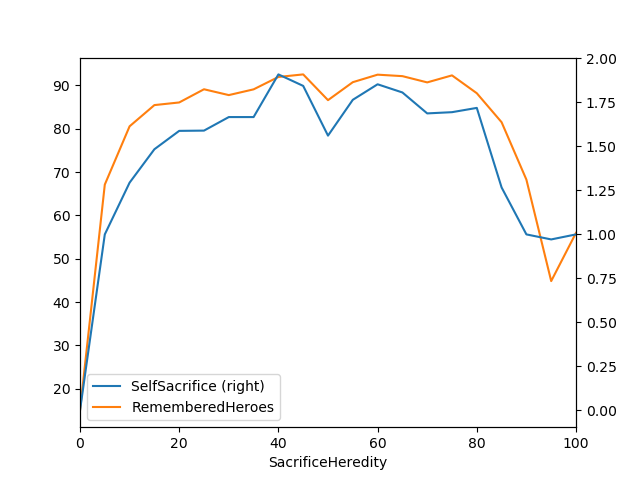
\includegraphics[width=0.6\textwidth]{Hered_a50}
    \caption{}
    \label{fig:h}
    \end{figure}


















\section{Two-tier model: mathematical analysis}


%%%% REDO ENTIRELEY
\subsection{Self-sacrifice}
%% OOPS ESS ?
For would-be martyrs $M$, the situation can be approached as in \textbf{Section \ref{sec_exo_math}}: the question comes down
to whether a non-trivial set of ESS strategies comprising a proportion $f$ of agents engaging in
self-sacrifice with probability $p$ can emerge\footnote{And $1-f$ agents not doing so.},
and meet the requirements of equation (\ref{eq:grandchildren}).

Total social admiration $A$ is now however \emph{endogenous}, as it is determined by how much
non-martyrs $\overline{M}$ engage in second-order signaling (honoring $h$):
%% meme approx implicite qu'avant : comme les martyrs meurent ... ils sgl pas la
%% SERAIT BIEN D'AVOIR DES NIVEAUX DE A ==> NIVEAUX DE f => NIVEAU DE P ...
%% ===> AU MOINS DANS LA "BRIEF DISCUSSION"
\begin{equation}
    \label{eq:A_h}
        A = \sum_{h(\overline{M}) \geq V_T}{h(\overline{M})}
\end{equation}

At (potential) equilibrium, $A$ will thus be determined by (potential) equilibrium levels
of honoring by patriots $P$ and non-patriots $\overline{P}$ and how high 
\emph{VisibleThreshold} $V_T$ is set. This, in turn, should determine
 if a self-sacrifice ESS is possible,
and, if so, at what proportion of martyrs $f$ can emerge at equilibrium, as before. Both
signals are thus connected via equation (\ref{eq:grandchildren}), which
can be tentatively rewritten according to equilibrium levels:

\begin{equation}
    \tag{\ref{eq:grandchildren}b}
    R_+(h_{P},h_{\overline{P}},f)*\beta(p) = r
\end{equation}
%%% Moui, ou meilleure equation pour signal 1 ===> niveau f...
%%% Bon ca devrait etre les eq quantites la: OSEF...

\subsection{Honoring and social score}

This is motivation to investigage the possibilty of an honoring equilibrium. Honoring $h$
and demand $d$ serve as bases for establishing friendships, which are mutually beneficial
(as controlled by \emph{FriendshipValue} $F$). However, intergroup conflict raises the stakes:
friends may be true patriots, to one's benefit (as controlled by \emph{PatriotFriendBonus} $P$),
or not be, leading to the possibility of betrayal with probability $t$ (\emph{NbTraitors})
and at potentially enormous cost $DC$ (\emph{DenunciationCost}).
%% WATCH OUT FOR NAMES

A patriot individual characterzied by $d$ and $h$, who obtains a number of friends $k$ on the
bases of these (genetic) characteristics will see his social score vary according to:

\begin{equation}
    \label{e:score}
    \mathbf{E}(\Delta_P(d,h)) = k*F + k_{P}*P - k_{\overline{P}}*t*DC
\end{equation}

In contrast, a non-patriot individuals also stand to gain \emph{Judas} $J$ if and when they
betray their friends:

\begin{equation}
    \tag{$\overline{\ref{e:score}}$}
    \label{e:score_NP}
    \mathbf{E}(\Delta_{\overline{P}}(d,h)) = k*F + k_{P}*P - k_{\overline{P}}*t*DC + t*J
\end{equation}



\subsection{Equilibrium when $t\leq \frac{F}{FC}$}
\label{s:null_ESS}

%%%%%%%%%%%%%%%%% FALSE !!!!!







%%%%%%%%%%% FALSE



Let us suppose that 
%honoring has reached some sort of stationary state, and that 
% = hyp champ constant ??
%%% JUSTIF ===> cf Maynard Smith maybe ?
individuals of the same quality all signal at the same level $s_{P}$ or $s_{\overline{P}}$,
and have equal demand $d_P$ or $d_{\overline{P}}$ (noted $d$ when there is no ambiguity).

Since individuals encounter patriots and non-patriots with equal probability,
and simply chooses whether or not to accept them based on $d$ (potential friends
are not ranked), a patriot with demand $d$ can be in one of four situations
%, dependingon where $d$ is situated with respect to $s_{P}$ or $s_{\overline{P}}$
(where $k$ notably depends on $d$ and time allocated to encountering
potential partners):

\begin{table}[h]
    \centering
    \begin{tabular}{|c || c c|} 
        \hline\
        $\mathbf{E}(\Delta_{P}(d,h))$ & $d \leq s_{\overline{P}}$ & $d>s_{\overline{P}}$\\ [1ex] 
        \hline\hline
        $d \leq s_{P}$ & $\frac{k}{2}*(2F+P-t*DC)$ & $k*(F+P)$ \\ [0.5ex]
        $d>s_{P}$ & $k*(F-t*DC)$ & $0$ \\ [0.5ex]
        \hline
    \end{tabular}
    \caption{Expected social score (patriot)}
\label{t:demand}
\end{table}
%rmq: bof alignment

When $t$ is sufficiently small, \textbf{Table \ref{t:demand}}'s first three cells
are strictly positive:
%%%%%%%%%%%%%%%%%%%% FALSE !
when betrayal is sufficiently improbable, friendship can always be expected to pay off for
patriots - as well as for non-patriots, since $\mathbf{E}(\Delta_{\overline{P}}(d,h)) 
\geq  \mathbf{E}(\Delta_P(d,h))$\footnote{At least when h is small - see after}.
For both, the the optimal "strategy" is thus $d=0$.
In addition, since honoring is costly, the best
response to $d=0$ is to not invest in honoring:

\begin{equation}
    \label{e:null_ESS}
    t \leq \frac{F}{DC} \implies \textnormal{
        ($d=0$, $h_P=0$, $h_{\overline{P}}=0$) is the only 
        NE\footnote{Nash equilibrium.}}
% Ou ailleurs: la premiere fois que NE utlise... cf section maths avant
\end{equation}

With typical parameter values, when \emph{NbTraitors} is smaller than $10\%$, no second-order signal
- and therefore no first-order signal - should emerge.
%% Ou plus tard / avant --> en lien avec les simu

\subsection{"Honest" equilibrium when $t \geq \frac{2F+P}{DC}$}
\label{s:h_ESS}

%%%% HONEST ==> in that informative...


When $t$ is sufficiently large, both cells on the left of \textbf{Table \ref{t:demand}} 
are negative: patriots cannot afford to have any non-patriot friends. Let us assume, following the first-version of the proposed simulation, that $s_{\overline{P}}$ is
bounded by \emph{MaxOffer} $MO$, and that non-patriots and patriots pay the same cost
for signaling.

For patriots, it is then always better to have $d > MO$ then $d \leq MO$. Indeed, in the latter
case where all patriots have demand $d < MO$, we are in a domain which is beneficial
for non-patriots: they stand to gain more from signaling (by potentially betraying),
at no extra cost. Thus, if $d < MO$, we expect $s_{\overline{P}} 
\geq s_P$\footnote{And $d_{\overline{P}} \leq d_P$}: the optimal situation represented
by \textbf{Table \ref{t:demand}}'s top right cell is unattainable, and, on average, patriots
stand to lose from friendship.

Conversely, if $d > MO$, patriots either obtain no friends or only patriot friends and
thus stand to benefit. Any stratetgy $d^+$ verifying $d^+>MO$ thus weakly dominates any other strategy $d^-$,
where $d^- \leq MO$.

Yet, as evoked in introducing equation (\ref{e:score}), an individual's number of friends $k$
depends on $d$. Given two demands above $MO$, the smaller is always best, since decreasing 
demand can only lead to increasing number of (patriotic) friends. For patriotic individuals,
the optimal strategy is thus the smallest available $d$ which is larger than $MO$,
which we will note $d = MO^{+}$.

%%%% EN FAIT C'est D = MO ?? 
%%% math : D = MO // simu : D = MO + erreur...
%%% REVENIR PLUS TARD : DISHONEST SGL !!!
%% (implicit assumption : can distinguish >= than can sgl)

Let us assume in addition that individuals have ample opportunity to meet potential friends,
forming $Max_F$ friendships when possible, at cost $c$,
and that $c * MO^+ < Max_F * (F+P)$\footnote{Otherwise signaling is never beneficial
and the only equilibrium is trivially (0,0,0).} . 
Patriots stand to gain from signaling at levels above of $MO$, and for them,
the optimal stratetgy is thus $MO^{+}$, following the same reasoning as above.

Non-patriots, however, can only attract other non-patriots:

\[ \mathbf{E}(\Delta_{\overline{P}}(d,h)) = k*(f - t*DC +t*J) \]

\[ \mathbf{E}(\Delta_{\overline{P}}(d,h)) \geq 0 \iff t \leq \frac{F}{DC-J} \]

In practice, the latter condition is incompatible with the one presented at the beginning
of this section, since, with typical values, $\frac{F}{DC-J} = \frac{2}{15}$ and 
$\frac{2F+P}{DC} = 0.3$. Thus:

\begin{equation}
    \label{e:h_ESS}
    t \geq \frac{2F+P}{DC} \implies \textnormal{
        ($d=MO^{+}$, $h_P=MO^{+}$, $h_{\overline{P}}=0$) 
        is the only NE}
\end{equation}

When \emph{NbTraitors} is greater than 30\%, a purely honest equilibrium should thus
emerge at the second-order - leading to self-sacrifice at a level 
corresponding to $A = MO^+ / 2$, since only half the population honors martyrs.
%%% DISHONEST / uninfo because of DEMAND GENE


\subsection{Dishonest equilibrium when $t \geq \frac{2F+P}{DC}$}
\label{s:_ESS}

%%% DISHONEST / uninfo because of DEMAND GENE


In practice not so much: 
- some dishonest, and not because stabilize at a level below permitted by J: cf \dots
- RemT = "more optimal" than expected

%%%% EN FAIT C'est D = MO ?? 
%%% math : D = MO // simu : D = MO + erreur...
%%% REVENIR PLUS TARD : DISHONEST SGL !!!
%% (implicit assumption : can distinguish >= than can sgl)


%%% DISHONEST / uninfo because of DEMAND GENE






%%%%%%%%%%%%%% BONUS : calcul noise / uncertainty / explo...













\subsection{$\frac{F}{DC}<t<\frac{2F+P}{DC}$}
%\label{s:relou_ESS}
%%%% COMMENCER ICI : relou ???


%When this is not the case, the question of whether $\mathbf{E}(\Delta_{P}(d^-,h))$ is positive
%notably comes down to whether or not the (patriot) individual has non-patriot friends or not.
%Let us assume, following the first-version of the proposed simulation, that $s_{\overline{P}}$ is
%bounded by \emph{MaxOffer} $MO$.

%We can distinguish two cases. Either $d \leq MO$, and the patriot individual has no way
%of distinguishing between potential friends. Since $\mathbf{E}(\Delta_{\overline{P}}(d,h)) 
%\geq  \mathbf{E}(\Delta_P(d,h))$, non-patriots stand to gain more from signaling, at no
%extra cost:
%it should follow that at equilibrium, their investment in honoring should be at least that
%of patriots (and their demand smaller). In other words, when $d<MO$,
%$s_{\overline{P}} \geq s_P$ and it is impossible for patriots to be in the optimal situation
%represented on the top right in \textbf{Table \ref{t:demand}}.


%%% PREDICTION : depend pas de P ????










%%%%%%%%%%%%% RADICALIZATION
%%%%%%%%%%%%%%%%%%%%%%%%%%---> (re)mettre DC mode apres...









\section{Second sacrifice model}
%/"Endogenous" model...



%%% En principe a refaire avec JB...
\begin{figure}[h]
    \centering
    \includegraphics[width=0.6\textwidth]{AP_MO50}
    \caption{}
    \label{fig:50}
    \end{figure}

%%% Sature encore a REMH = 80 : en-dessous non ??
%%%%%%%%%%%%%%%% ah a peine plus grand le second ?
%%%%%%%%%%%%%%%%%%%%%%%%%%%%%%%% non
%%% encore "un peu" informatif...
%%% a updater once aver resultats lame23
    \begin{figure}[h]
        \centering
        \includegraphics[width=0.6\textwidth]{AP_MO75}
        \caption{}
        \label{fig:75}
        \end{figure}
    




\section{Limitations}
%Oops NonPatriots that actually self-sacrifice....
%% HERE MORE LIKE ?

\chapter{Perspectives}
%%\section{Limitations}
%Oops NonPatriots that actually self-sacrifice....

%\part*{Bibliography}
%take out III ?
%\bibliographystyle{plain}
%\bibliography{/home/tom/Documents/Stage/Memoire/Memoire}

%\cite{dessalles_optimal_2014}
\bibliographystyle{apacite}
\bibliography{Memoire}
%%%%%%%%%%%%%%% oops url too long...

\appendix
%\part{Appendix}
%Take out IV?

\chapter{Python stuff}
\label{a:scripts}
\chapter{Mathematical demonstrations}

\section{Exogenous model}
%\subsection{RemTH}
\subsection{$\beta(p)$}
\label{beta}



Disregarding the effects of natural selection (which are the same for all individuals 
here\footnote{And will therefore appear on both sides of an equation comparing
the benefits of either strategy such as (\ref{eq:grandchildren}).}),
 an individual who bears a $\bf{SelfSacrifice}$ gene of relative value $p$, has a probability $p$ of dying in his first year
 (before being able to foster any descendants), a probability $(1-p)*p$ of dying at age $1$ ...
 a probability $(1-p)^{n}*p$ of dying at age $n<M$ ... and is certain to die at age $M$, should
 he or she reach it. His/her expected life span is thus:
 \[ ELS = p*0 + (1-p)*p*1 + ... + (1-p)^{M-1}*(M-1) + (1-p)^M*M \]

 \begin{figure}[h]
    \centering
    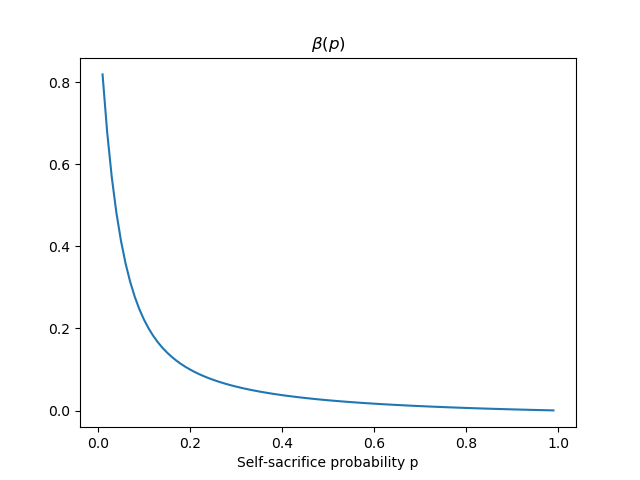
\includegraphics[width=1\textwidth]{Beta}
    \caption{Loss of expected life-span due to self-sacrifice.}
    \label{fig:beta}
\end{figure}

Let $f \colon \mathbf{R} \to \mathbf{R}$ be the polynomial function defined by the expression:
\[ f(x) = \sum_{n=0}^{M-1} p*(1-p)^n*x^n + (1-p)^M*x^M \]

By deriving $f$, one can note that:
\begin{equation}
    ELS = f'(1)
\label{eq_ELS_f}
\end{equation}

$f(x)$ involves a geometric sum and can be simplified to (when $(1-p)*x$ is different than 1):
\[ f(x) = p* \frac{1 - ((1-p)*x)^M}{1-(1-p)*x} + ((1-p)*x)^M \]

For $x\neq\frac{1}{(1-p)}$ ($p=1$ trivially yields $ELS=0$):
\[ f'(x) = p * \frac{-M(1-p)^Mx^{M-1}*(1-(1-p)x) + (1-p)*(1-((1-p)x)^M)}{(1-(1-p)x)^2} + M(1-p)^Mx^{M-1} \]

And thus:
\[f'(1) = p * \frac{(-M(1-p)^M*p + (1-p)*(1-(1-p)^M)}{p^2} + M(1-p)^M \]

\begin{equation}
    f'(1) = \frac{(1-p)*(1-(1-p)^M)}{p}
\label{eq_f'}
\end{equation}

Combining these two expressions for $f'(1)$ proves equation ($\bf\ref{eq_beta}$). \textbf{Figure \ref{fig:beta}} shows
$\beta(p)$ for $p$ between 0 and 1. Factoring in natural selection, an individual's expected life span is therefore equal to: $\alpha*\beta(p)*M$.




\subsection{$R_{+}(A)$}
\label{ss:R+}
In $\bf{Selectivity}$ mode, individuals obtain reproductive potential $R$ according to their
$\bf{Reproductive\_points}$ $RP$: each individual obtains a rank $k$
according to $RP$, and receives reproductive potential:
\[ R = \frac{r}{2} * (\frac{S}
{(S*k + N')*log(1+S)} + \frac{S}{(S*(k+1) + N')*log(1+S)}*N') \]

where $N'<N$ is the number of eligible parents (non-martyrs) and $S$ is equal to \emph{Selectivity}
(the average reproductive potential over eligible parents being \emph{ReproductionRate} $r$).
When $N \gg 1$, $R$ verifies:
\begin{equation}
    R \in [R_{min};R_{max}], \textrm{with } R_{max} \approx \frac{S*r}{log(1+S)} 
    \textrm{ and } R_{min} \approx
    \frac{R_{max}}{1+S}
\label{eq:ReproPot}
\end{equation}

With typical parameters ($S=10$ and $r=15\%$), we obtain: $R_{max} \approx 63 \%$ and 
$R_{min} \approx 5,6 \%$.

In a case where a negligible proportion $f$ of individuals engage in
self-sacrificial behavior (which is assured to end up in their martyrdom), their children each
receive, on average:
\begin{itemize}
\item reproductive potential $r$, when $A < A_{min}$ ;
\item $R_{+}(A,f)$ otherwise, as seen in \textbf{Section \ref{ss: exo_existence}}.
\end{itemize}

When $N \gg 1$, expected $R_+(A,f)$ is equal to the average between the "luckiest" ($k=0$) and "unluckiest"
child, which is approximately:
\[ R_+(A,f) \approx \frac{S*r}{2*log(1+S)} * (1 + \frac{1}{S*f+1}*\frac{N}{N})\]

Which yields, for $f\ll 1$ (neglecting terms of order 2 and above in $f$):
\begin{equation}
    \tag{\ref{eq:R+}}
    R_+(A,f) \approx  \frac{S*r}{log(1+S)} * (1 - \frac{S*f)}{2}) = 
    R_{max}*(1-\frac{S*f}{2})
\end{equation}

\subsection{Nash equilibrium}
\label{ss_e_a:ESS}
%% Ah non...

 
\end{document}

%Tous les calculs sont faits en moyenne / esperance... pas precise a chaque fois ?


%Using (\ref{eq:min_ESS_e}), we can further deduce that for such an ESS to exist,
%we must have:

%\[A \geq A_{min}=\frac{RGT*f*log(1+S)*(M*log(1+S)+S)}{(M*log(1+S)+S)*S - S^2*f}  \]
    
%\[f \leq f_{max} = \frac{A*S(M*log(1+S)+S)}{RGT*log(1+S)+S*A}\]
